
    \section{Gestione della Memoria}
    La memoria é oggi a basso costo, e con trend in diminuzione, questo fa si che le applicazioni usino sempre piú memoria,
    se ogni processo dovesse gestire la propia memoria, ogni processo userebbe semplicemente tutta la memoria disponibile,
    questo porterebbe all'assenza della multiprogrammazzione che é un aspetto essenziale per il corretto funzionamento del
    sistema operativo, si potrebbe imporre dei limiti di memoria a ciascun processo, diventa peró difficile per un programmatore
    scrivere un processo che rispetti tali limiti, quindi ogni sistema operativo deve avere un sistema di gestione della memoria
    cercando di dare l'illusione ai processi di avere tutta la memoria, la soluzione é quella di usare il disco come buffer
    per memoria, questa gestione di I/O é ovviamente piú lenta del processore, per cui il SO deve pianificare lo swap
    \subsection{Requisiti}
    \begin{itemize}
        \item Rilocazione : importante che ci sia aiuto hardware, aiuto, non gestione diretta per cui sistema operativo e hardware collaborano
        \item Protezione : importante che ci sia un aiuto hardware
        \item Condivisione
        \item Organizzazione logica
        \item Organizzazione fisica
    \end{itemize}
    \subsubsection{Rilocazione}
    Il programmatore non sa e non deve sapere in quale zona della memoria il programma verrá caricato :
    \begin{itemize}
        \item potrebbe essere swappato su disco, e al ritorno in memoria principale potrebbe essere caricato in un'altra zona
        \item potrebbe anche non essere contiguo, oppure con altre pagine in RAM e altre in disco
        \item in questo contesto, si intende chi usa l'assembler o il compilatore
    \end{itemize}
    I riferimente alla memoria devono essere tradotti nell'indirizzo fisico : preprocessing, run-time,se run-time occrre supporto hardware
    \begin{figure}[H]
        \centering
        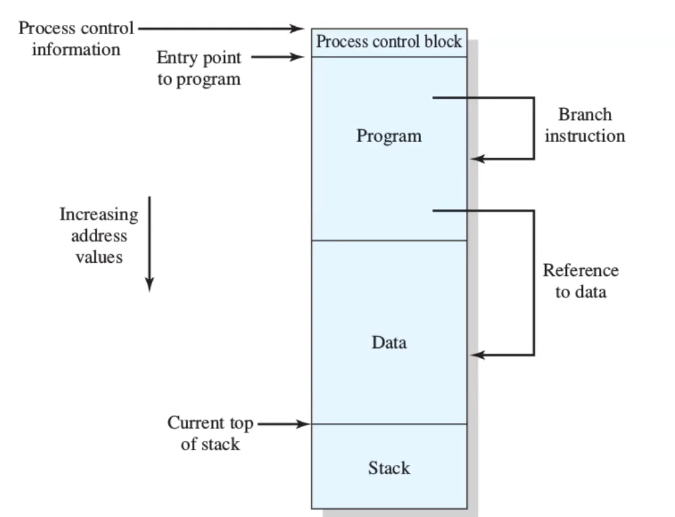
\includegraphics[width=0.75\textwidth]{immagini/RilocazioneIndirizziNeiProgrammi}
        \caption{Rilocazione}
    \end{figure}
    un processo ha una zona con il programma in liguaggio macchina, e una zona con i dati, e una zona con lo stack, la sua parte iniziale
    é il PCB, gli indirizzi che possiamo avere sono indirizzi di salto oppure referenze a variabili, tutti questi inidirizzi
    devono essere ricalcolati.
    \subsubsection*{Indirizzi nei programmi}
    \begin{figure}[H]
        \centering
        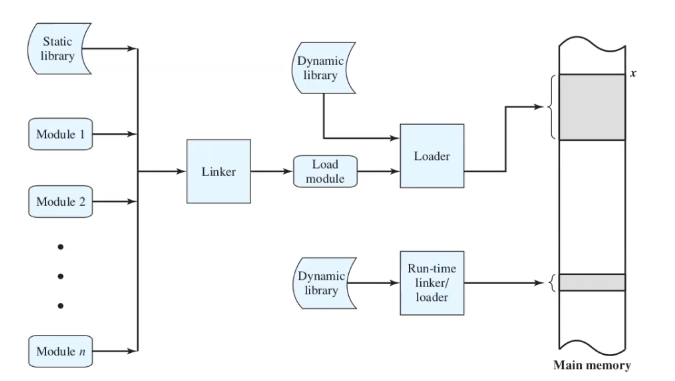
\includegraphics[width=0.75\textwidth]{immagini/Indirizzi nei programmi}
        \caption{Indirizzi nei programmi}
    \end{figure}
    Per capire come avviene la rilocazione dobbiamo prima precisare... Un programma eseguibile viene prima scritto
    in moduli, uno di questi moduli ha il main, quindi ci sono tanti moduli scritti dal programmatore oppure librerie
    , ognuno di questi moduli viene compilato separatamente, ed per ogni modulo viene creato un file oggetto, tutto
    questo viene collegato attraverso il linker in modo da creare un file eseguibiler (nell'esempio Load module),
    poi c'é il loader che carica il file eseguibile in memoria, nel fare questo ci potrebbe essere bisogno di alcune librerie dinamiche
    \begin{figure}[H]
        \centering
        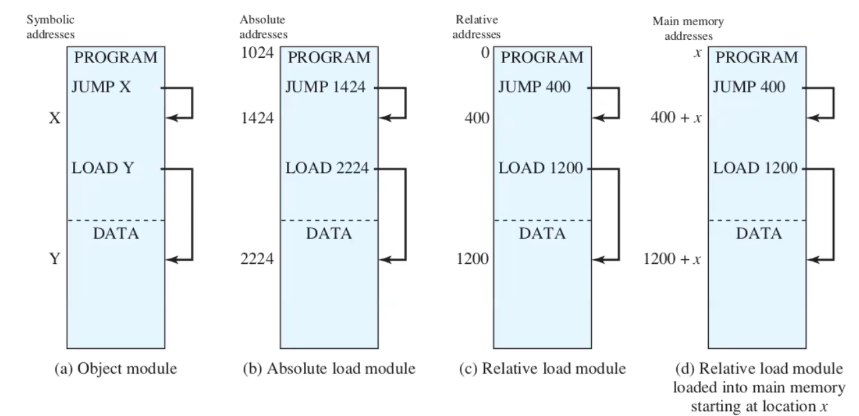
\includegraphics[width=0.75\textwidth]{immagini/IndirizziInMemoria}
        \caption{Effettivo in memoria}
    \end{figure}
    Il risultato é mostrato nell'immagine, ogni singolo modulo ha la sua parte di programma e la sua parte di dati,
    sostanzialmente il programma contiene soltanto indirizzi simbolici, quando peró viene trasformato in un file eseguibile
    abbiamo 2 possibilitá:
    \begin{itemize}
        \item Indirizzo Assoluto : Lui sa che deve cominciare a 1024, e se deve saltare a 1424, il loader deve caricare il programma all'indirizzo 1024 altrimenti non funziona.
        \item Indirizzo Relativo : Con gli inderizzi relativi, si puó suppore di partire da 0, e nel caso di un salto scrivo solo l'indirizzo rispetto all'inizio del programma.
    \end{itemize}
    \subsubsection*{Tipi di Indirizzi}
    \begin{itemize}
        \item \textbf{Indirizzi Logici} : vengono usati dal programmatore, sono indirizzi simbolici, non sono reali, sono rilocati
        \item \textbf{Indirizzi Fisici} : sono gli indirizzi reali, sono quelli che vengono usati dal processore
        \item \textbf{Indirizzi Relativi} : il riferimento é espresso come un un spiazzamento rispetto ad un punto di riferimento.
    \end{itemize}
    \begin{figure}[H]
        \centering
        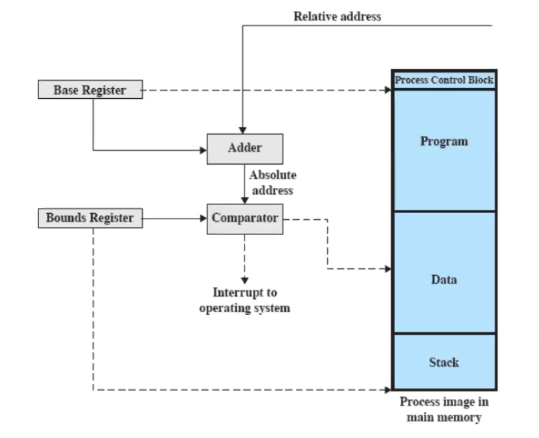
\includegraphics[width=0.75\textwidth]{immagini/RilocazioneConHardware}
        \caption{Tipi di Indirizzi}
    \end{figure}
    Nel caso di indirizzi relativi, l' hardware della macchina sa che se per esempio abbiamo un salto a 100, allora
    l'hardware sa che deve sommare 100 all'indirizzo base (Es. 6000), quindi l'indirizzo fisico sará 6100, inoltre c'é una
    fase di controllo per rimanere nei limiti di memoria, e fondamentale che ogni volta che il sistema operativo carica il
    processo il sistema operativo deve preoccuparsi di mettere l'indirizzo corretto nel base register.\\

    I registri usati sono:
    \begin{itemize}
        \item Base Register : contiene l'indirizzo base del processo.
        \item Limit Register : contiene l'indirizzo di fine del processo.
    \end{itemize}
    I valori per questi registri vengono settati nel momento in cui il processo viene posizionato in memoria, mantenuti nel PCB del processo,
    fa parte del passo 6 del process switch e non vanno semplicemente modificati occore propio modificarli.
    \subsubsection{Protezione}
    I processi non devono poter accedere alla locazione di memoria di memoria di un'altro processo, a meno che
    non sia stato esplicitamente condiviso, A causa della rilocazione non puó essere fatto a tempo di compilazione,
    pertanto serve un supporto hardware.
    \subsubsection{Condivisione}
    La condivisione deve essere possibile, permettere a piú processi di accedere alla stessa locazione di memoria, solo se é effettivamente
    utile allo scopo perseguito, c'é anche casi in cui é il sistema operativo in maniera trasparente, il caso tipico é quando
    si seseguono piú processi eseguendo lo stesso codice sorgente, quindi lo metto in RAM una volta sola.
    \subsubsection{Organizzazione Logica}
    A livello hardware, la memoria é organizzata in modo lineare, A livello software , i programmi sono scritti in moduli,
    per cui il SO deve offrire tali caratteristiche, facendo da ponte tra la prima visuale (moduli) e la seconda (lineare).
    \subsubsection{Organizzazione Fisica}
    L' organizzazione fisica é quella che si occupa del flusso di dati tra RAM e la memoria secondari, questa non é una
    cosa lasciata al programmatore, se per esempio io scrivo un programma che necessitá di 1GB di ram ma il sistema
    operativo me ne assegna 500MB, una volta il programmatore doveva usare l'overlay per suddividere il programma in
    pezzi e gestire lo swap tra ram e disco in maniera manuale, oggi il sistema operativo si occupa di tutto ció.
    \subsection{Partizionamento}
    Uno dei primi metodi per gestire la memoria é il partizionamento, la memoria viene divisa in partizioni, esso
    puó essere di diversi tipi:
    \begin{itemize}
        \item \textbf{Partizionamento Fisso} : la memoria é divisa in partizioni di dimensione fissa.
        \item \textbf{Partizionamento Dinamico} : la memoria é divisa in partizioni di dimensione variabile.
        \item \textbf{Paginazione Semplice} : la memoria é divisa in pagine di dimensione fissa.
        \item \textbf{Segmentazione Semplice} :
        \item \textbf{Paginazione con memoria virtuale} :
        \item \textbf{Segmentazione con memoria virtuale} :
    \end{itemize}
    \subsubsection{Partizionamento Fisso Uniforme}
    Quando accendo il sistema operativo, tra le cose che vengono fatte il SO divide la memoria in partizioni di dimensione
    fissa, 1 é riservata al kernel, le altre sono per i processi, l'idea é quella di mettere al loro interno i processi
    che peró non possono superare la partizione assegnata all'inizio, chiaramente il SO puó decidere se sospendere
    e quindi spostare il processo sul disco, in questo caso era il programmatore a dover essere sicuro di non sforare
    la partizione assegnata.
    \subsubsection*{Problemi}
    un programma potrebbe non entrare in una partizione, questo porta anche ad un uso inefficiente della memoria, perché
    porta al fenomeno della frammentazione interna.
    \subsubsection{Partizionamento Fisso Variabile}
    Nel partizionamento variabile comunque le partizioni vengono assegnate una sola volta, ma la dimensione delle partizioni
    é variabile, questo permette di mettere i processi piú leggeri in partizioni piú piccole.
    \subsubsection*{ALgoritmo di Posizionamento}
    Da momento in cui ho partizioni di dimensioni variabili, mi devo preoccupare di dove mettere i processi, una scelta
    é quella di avere una coda per partizione , oppure ho una unica coda e mano a mano assegno alla partizione che spreca
    meno spazio, se uso la coda unica posso fare delle ottimizzazioni nel senso che piuttosto che non far eseguire un
    processo lo carico in memoria, anche se spreco un po' di memoria.
    \begin{figure}[H]
        \centering
        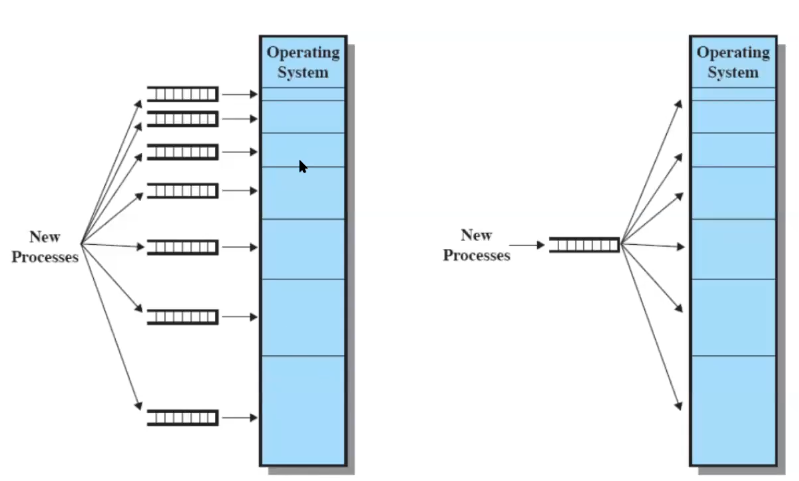
\includegraphics[width=0.75\textwidth]{immagini/partizionamento}
        \caption{Partizionamento Variabile}
    \end{figure}
    \subsubsection*{Problemi Irrisolti}
    C'é un numero massimo di processi in memoria principale dettato dal fatto che il numero di processi non puó superare
    il numero di partizione, inoltre la gestione della memoria risulta comunque inefficiente se ho tanti processi piccoli.
    \subsubsection{Partizionamento Dinamico}
    Le partizioni variano sia in misura che in quantitá, la dimensione delle partizione varia in base alla dimensione 
    del processo.
    \subsubsection*{Esempio}
    \begin{figure}[H]
        \centering
        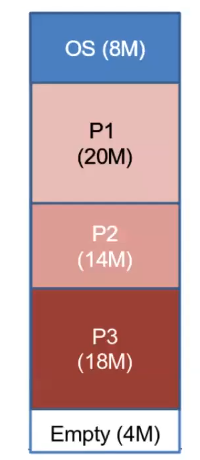
\includegraphics[width=0.25\textwidth]{immagini/EsempioPartizionamentoDinamico}
        \caption{Partizionamento Dinamico}
    \end{figure}
    Supponiamo che arrivino in sequenza tre processi, p1=20MB, p2=14MB, p3=18MB, stiamo
    assumendo che chiaramente stiamo usando indirizzi relativi, in una memoria da 56M
    resta un blocco da 4MB, se arriva un processo da 5MB, il sistema operativo deve fare una
    scelta, supponiamo che il processo da 5MB sia il processo p4 e sia piú importante di p2
    \begin{figure}[H]
        \centering
        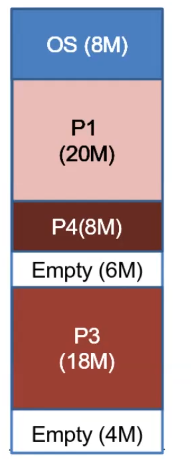
\includegraphics[width=0.25\textwidth]{immagini/EsempioPartizionamentoDinamico2}
        \caption{Partizionamento Dinamico}
    \end{figure}
    quello che succede é che si lascia uno spazio vuoto di 6MB, p2 chiaramente viene copiato
    sul disco in attesa che venga richiamato, ora peró vogliamo far eseguire p2 che é piú importante
    di p1 copiamo p1 sul disco e carichiamo p2 in memoria, ora abbiamo un ulteriore spazio vuoto di 6MB
    \begin{figure}[H]
        \centering
        \includegraphics[width=0.25\textwidth]{immagini/EsempioPartizionamentoDinamico3}
        \caption{Partizionamento Dinamico}
    \end{figure}
    si nota che ci sono 16MB di spazio vuoto, se arriva un processo da 10MB, non
    lo posso eseguire perché la memoria non é contigua.
    \subsubsection*{Problemi}
    La frammentazione esterna é un problema, che peró si puó risolvere con la compatazzione. \\

    se ho piú blocchi liberi, ed arriva un processo che potrebbe entrare in uno di questi blocchi, il sistema operativo
    utilizza un algoritmo per scegliere il blocco in cui mettere il processo, l'algoritmo puó essere:
    \begin{itemize}
        \item First Fit : metto il processo nel primo blocco che trovo
        \item Best Fit : metto il processo nel blocco piú piccolo che trovo
        \item Worst Fit : metto il processo nel blocco piú grande che trovo
    \end{itemize}
    \subsubsection*{Best Fit}
    l'algoritmo Best Fit ad una prima valutazione potrebbe sembrare il migliore, ma in realtá é il peggiore, perché
    lascia tanti piccoli blocchi liberi, che non possono essere usati.
    \subsubsection*{First Fit}
    \begin{enumerate}
        \item scorre la memoria dall'inizio; il primo blocco con abbastanza spazio viene usato
        \item é molto veloce
        \item tende a riempire solo la prima parte della memoria
        \item A conti fatti era il migliore
    \end{enumerate}
    \subsubsection{Next Fit}
    Next Fit é una variante di First Fit, la differenza é che Next Fit ricorda dove ha finito l'ultima volta, e riparte
    dall'ultima appena asseggnate per evitare che solo la prima parte della memoria venga usata, assegna piú spesso
    l'ultimo blocco di memoria.
    \begin{figure}[H]
        \centering
        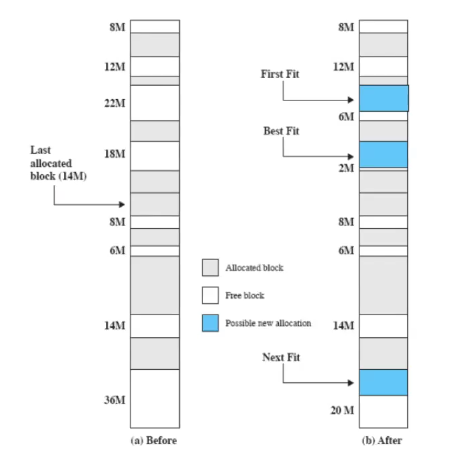
\includegraphics[width=0.75\textwidth]{immagini/AlgoritmiPartizionamento}
        \caption{Confronto tra algoritmi}
    \end{figure}
    \subsubsection{Buddy System}
    Il Buddy system é ancora partizionamento, in questo caso é un compromesso tra partizionamento fisso e dinamico,
    é ancora usato nei sistemi operativi moderni, esempio : supponiamo che 2^U la dimensione di memoria di memoria
    a disposizione per l'utente e che \textbf{s} sia la dimensione di un processo, quello che fa il buddy system é
    dividere per 2 fino a che non si arriva alla dimensione tale che:
    \begin{equation}
        2^(X-1) <= s <2^x
    \end{equation}
    Una delle 2 porzioni é usata per il processo, L' invece serve per dare un lower bound, ovvero non si potranno creare
    partizioni troppo piccole, quando il processo finisce, se il buddy é libero, si uniscono.\\

    Esempio: supponiamo di avere un blocco da 1 MB, e che arrivi un processo da 100KB, quindi andiamo a dividere
    il blocco per 2, ed osserviamo di avere 2 blocchi da 512KB, il blocco é ancora troppo grande, ne prendiamo uno
    e lo dividiamo per 2, ottenendo 2 blocchi da 256KB, il blocco é ancora troppo grande, ne prendiamo uno e lo dividiamo
    per 2, ottenendo 2 blocchi da 128KB, il blocco adesso é della dimensione corretta perché se divido ancora per 2 i 2 blocchi
    risultanti saranno troppo piccoli per ospitare il processo,ci sará quindi una frammentazione interna di 28KB, supponiamo
    ora  che arrivi un processo da 240KB, vediamo che dalla divisione di prima é avanzato un blocco da 256KB e quindi
    quella partizione viene usata, ora supponiamo che arrivi un processo da 64KB, dividiamo il blocco da 128KB e selezioniamo
    uno dei due blocchi da 64KB, per ricreare le partizioni quando un processo termina, l'idea é quella di riaccoppiare i blocchi
    con i propri buddy, quindi se un blocco da 64KB termina, si unisce con il blocco da 64KB, e tutti e due devono derivare
    dallo stesso blocco da 128KB e cosi via fino a riformare il blocco da 1MB.
    \begin{figure}[H]
        \centering
        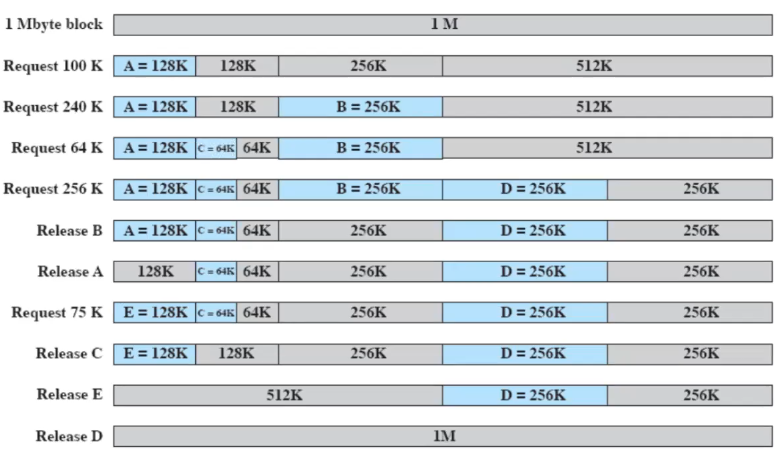
\includegraphics[width=0.75\textwidth]{immagini/BuddySystem1}
        \caption{Buddy System}
    \end{figure}
    Da notare che il buddy system si presta bene per essere rappresentato come un albero binario, quindi
    per migliorare la ricerca si implementava la ricerca tramite bynary search tree, in questo modo si evita di scorrere tutta
    la memoria.
    \begin{figure}[H]
        \centering
        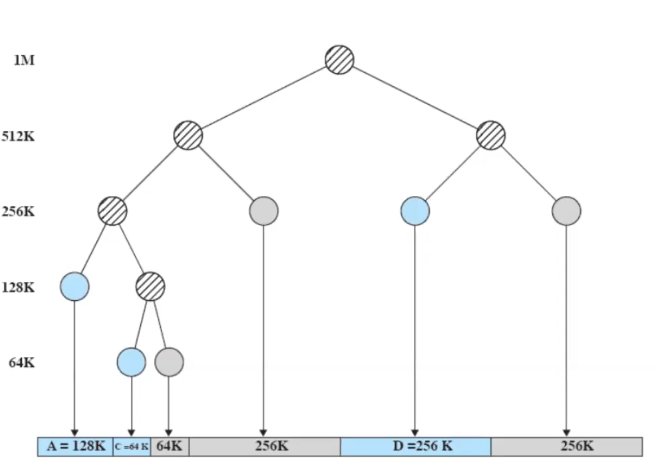
\includegraphics[width=0.75\textwidth]{immagini/BuddySystemAlbero}
        \caption{Buddy System}
    \end{figure}
    \subsection{Paginazione}
    \subsubsection*{Paginazione Semplice}
    Sia la memoria che i processi vengono divisi in pezzi di dimensione fissa e piccola (1KB), questo si fa sia
    con la RAM che con i processi, se un processo é grande 1MB viene diviso in 1024 pezzi (1KB), questi pezzi
    sono chiamati pagine per i processi, mentre i pezzetti di memoria sono chiamati frame, La cosa essenziale
    che ogni pagina per essere utilizzata deve essere collacata in un frame, la cosa interessante che pagine
    contigue non devono essere collocate in frame contigui, questo permette di evitare la frammentazione interna,
    tutto il processo é trasparente al programmatore, a questo punto serve che i sistemi operativi mantengano
    una tabella che mappi le pagine ai frame, questa tabella é chiamata Page Table, questo punto peró bisogna
    correggere gli indirizzi, per cui c'é bisogno di un supporto hardware.
    \subsubsection*{Esempio}
    Supponiamo che arrivi un processo \textbf{A} che richiede 4 frame, poi \textbf{B} da 3 frame, e poi \textbf{C} da
    4 frame, poi il processo \textbf{B } termina, quello che succederebbe se fossimo in partizionamento dinamico ed
    arrivasse un processo da 5 dovrei eseguire la compattazione, in questo caso invece posso usare i 3 frame che
    erano stati assegnati a \textbf{B} per il processo \textbf{D}, ed i restanti 2 frame li posso accodare a C.
    \begin{figure}[H]
        \centering
        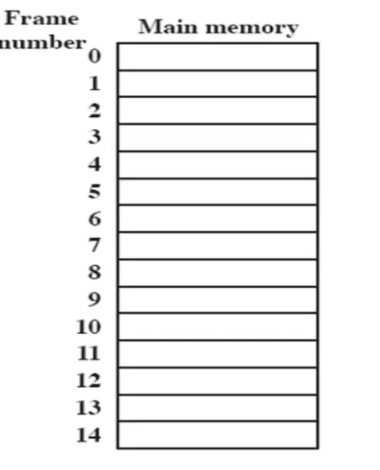
\includegraphics[width=0.5\textwidth]{immagini/PaginazioneEsempio1}
    \end{figure}
    \begin{figure}[H]
        \centering
        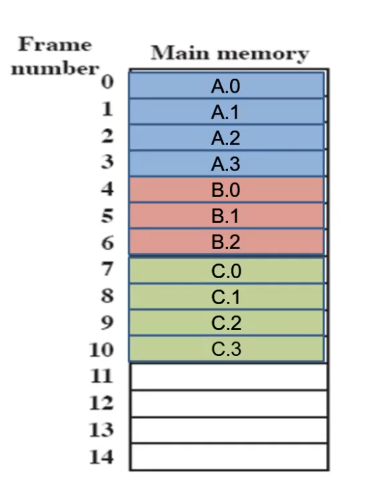
\includegraphics[width=0.5\textwidth]{immagini/PaginazioneEsempio1and2}
    \end{figure}
    \begin{figure}[H]
        \centering
        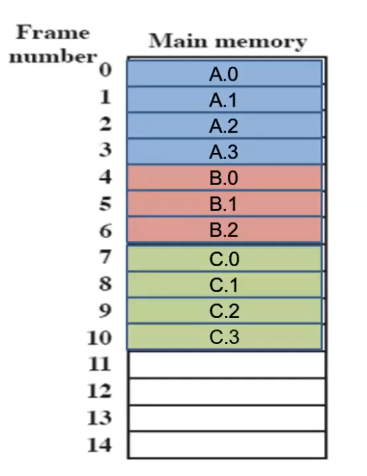
\includegraphics[width=0.5\textwidth]{immagini/PaginazioneEsempio2}
    \end{figure}
    \begin{figure}[H]
        \centering
        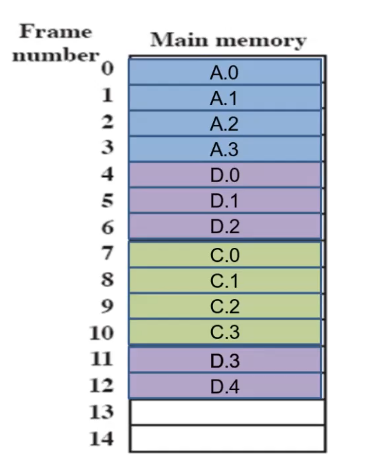
\includegraphics[width=0.5\textwidth]{immagini/PaginazioneEsempio3}
    \end{figure}
    Le tabelle risultanati sono:
    \begin{figure}[H]
        \centering
        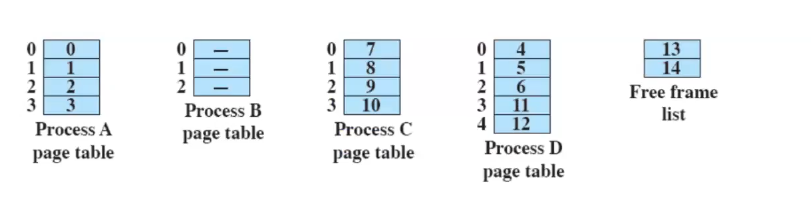
\includegraphics[width=0.75\textwidth]{immagini/PagineRisultanti}
        \caption{Tabelle delle pagine risultanti}
    \end{figure}
    \subsection{Segmentazione}
    \subsubsection*{segmentazione Semplice}
    La differenza tra segmentazione e paginazione é che la segmentazione divide i processi in segmenti di dimensione
    variabile, mentre la paginazione divide i processi in pagine di dimensione fissa, la differenza é che
    il programmatore a dover dividere il processo in segmenti(Sorgenti,Dati,\ldotsecc), dichiarando quali segmenti ci sono e qualé la loro dimensione
    a caricarli in memoria ed a risolvere gli indirizzi é il sistema operativo, sempre con l'aiuto dell'hardware.
    \subsection{Indirizzi Logici}
    Dobbiamo quindi considerare una rivisitazione degli indirizzi logici,
    con gli indirizzi relativi ad esempio, il programmatore sa che il suo programma inizia a 0, e che se deve saltare
    a 100, deve scrivere 100 poi é il sistema operativo che aggiunge l'offset necessari per andare
    all'istruzione corretta,Supponiamo quindi di avere un processo diviso in 3 pagine (notare che é presente
    la frammentazione interna), la prima cosa da fare quindi con un indirizzo é capire in quale pagina si trova dopo
    di che ho un offset rispetto all'inizio della pagina, devo andare ad usare la tabella delle pagine per capire dove
    si trova l'inizio del frame e sommare l'offset, il risultato é l'indirizzo fisico, in maniera analoga
    funziona anche per la segmentazione, da tenere presente che i segmenti hanno dimensione variabile.
    \begin{figure}[H]
        \centering
        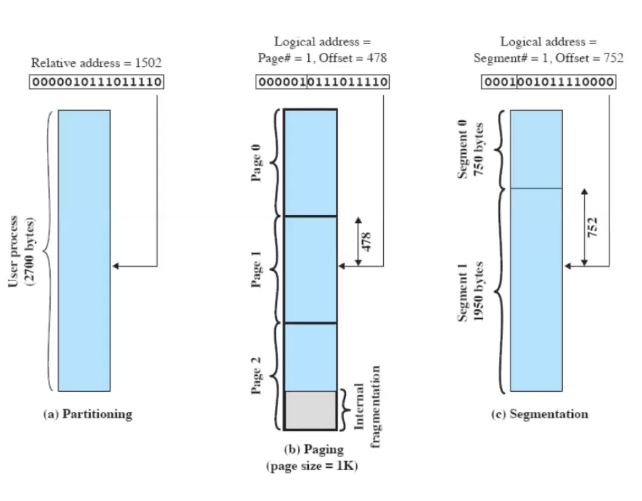
\includegraphics[width=0.75\textwidth]{immagini/IndirizziLogici1}
        \caption{Indirizzi Logici}
    \end{figure}
    \subsubsection*{Paginazione Esempio}
    Supponiamo di essere in una istruzione hardware e questa istruzione harware ha un indirizzo di 16 bit logico,
    quello che devo fare é ricavare l'indirizzo fisico,le dimensioni delle pagine sono sempre un potenza di 2
    allora lascio i primi 10 bit che sono usati per l'offset, mentre i 6 bit piú significativi sono usati per
    capire in quale pagina si trova l'indirizzo questo é vero perché abbiamo preso pagine di dimensione \begin{math}2^1^0\end{math}
    quindi per generalizzare se la dimensione della pagina é \begin{math}2^x\end{math} allora gli x bit meno significativi sono usati
    per l'offset, mentre i bit piú significativi sono usati per capire in quale pagina si trova l'indirizzo, quind una
    volta trovata la pagina, vado a sostituire il contenuto della tabella all'interno dei dei bit che prima erano
    riservati alla tabella, in sostanza i bit piú significativi all'inizio sono usati per contenere l'indirizzo per la
    tabella delle pagine che contiente i bit che servono per trovare l'indirizzo fisico.
    \begin{figure}[H]
        \centering
        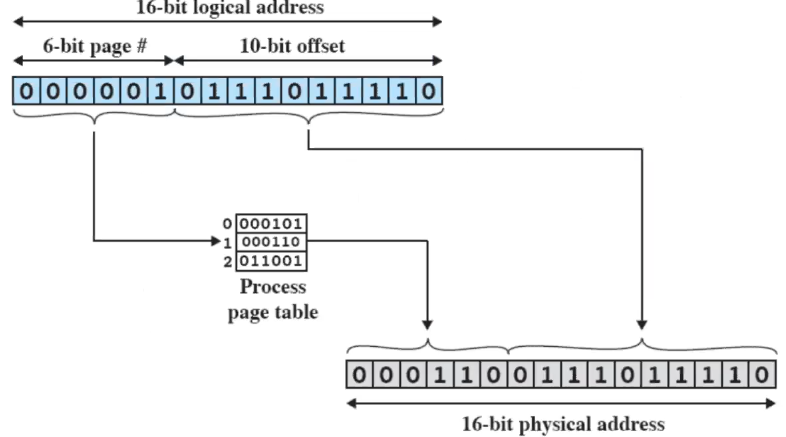
\includegraphics[width=0.65\textwidth]{immagini/funzionamentopaginazione1}
        \caption{}
        \label{fig:funzionamentopaginazione1}
    \end{figure}
    \subsubsection*{Segmentazione Esempio}
    Se voglio tradurre da indirizzo logico a indirizzo fisico, anche in questo caso la lunghezza massima dei segmenti é
    decisa dal sistema operativo, in questo caso siccome ogni segmento ha una dimensione varaibile devo andare a recuperare
    la posizione del segmento nella tabella dei segmenti, e sommare  i bit di offset, inoltre nella tabella é contenuta
    anche la lunghezza del segmento.
    \begin{figure}[H]
    \centering
    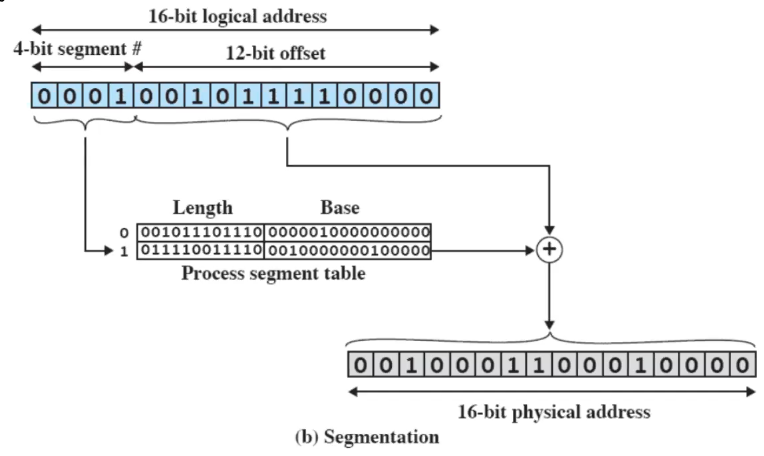
\includegraphics[width=0.65\textwidth]{immagini/indirizzologicosegmentazione}
    \caption{}
    \label{fig:indirizzologicosegmentazione}
    \end{figure}
    \subsection{Memoria Virtuale}
    I riferimenti alla memoria quindi sono indirizzi logici che devono essere tradotti in indirizzi fisici, con
    la paginazione e la segmentazione un processo puó essere diviso in piú parti é puó trovarsi in zone differenti
    della memoria, l'idea é che effettivamente non c'é la necessitá che tutto il processo sia in memoria principale,
    perché quello che serve effettivamente é che la parte del processo che é in esecuzione sia in memoria principale,
    tutto il resto puó essere sul disco,quindi il sistema operativo mette in memoria solo la parte del processo
    che é in esecuzione questo insieme di dati in memoria principale si chiama \textbf{resident set}, se la
    pagina peró non si trova in memoria principale, si verifica un \textbf{page fault}, il sistema operativo
    quindi chiama un interrupt che si occupa di andare a prendere la pagina mancante e metterla in memoria principale,
    fino a che la pagina non é in memoria principale il processo é blocked, quando effettivamente la pagina é effettivamente
    in memoria il processo viene sbloccato e puó continuare l'esecuzione, \textbf{quando il processo verrá eseguito bisognerá
    ri-eseguire l'istruzione che ha causato il page fault}.
    \subsubsection*{conseguenze}
    \begin{itemize}
        \item Ci possono essere molti processi in memoria principale perché basta una pagina in memoria principale
        \item Diventa molto probabile che ci sia un processo ready diminuendo l'idle del processore
        \item Posso eseguire un programma piú grande della memoria principale
    \end{itemize}
    \subsubsection*{Terminologia}
    La Memoria virtuale é uno schema di allocazione di memoria, in cui la memoria secondaria puó essere usata come se
    fosse memoria principale.
    \begin{itemize}
        \item Gli indirizzi usati nei programmi e quelli usati dal sistema sono diversi
        \item C'é una fase di traduzione automatica dai primi indirizzi (logici) ai secondi (fisici)
        \item La dimensione della memoria virtuale é limitata dallo schema di indirizzamento, oltre che
        dalla dimensione della memoria secondaria
        \item la dimensione della memoria principale, non influisce sulla dimensione della memoria virtuale
        \item \textbf{Indirizzo Virtuale} : indirizzo logico
        \item \textbf{Spazio degli indirizzi virtuali} : la quantitá di memoria virtuale assegnata ad un processo
        \item \textbf{Spazio degli indirizzi}: la quantitá di memoria assegnata ad un processo
        \item \textbf{Indirizzo Reale} : indirizzo fisico
    \end{itemize}

    \begin{figure}[H]
        \centering
        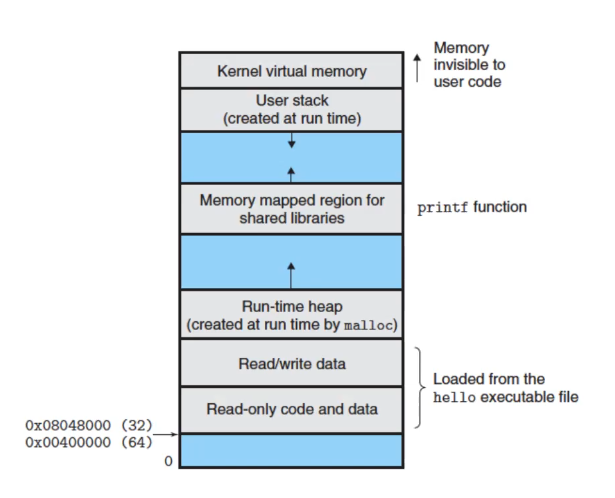
\includegraphics[width=0.65\textwidth]{immagini/comeunprocessovedelamemoria}
        \caption{come un processo vede la memoria}
        \label{fig:comeunprocessovedelamemoria}
    \end{figure}
    \subsubsection{Trashing}
    Il trashing é quando il sistema operativo perde piú tempo a fare swap tra memoria principale e secondaria per
    caricare le pagine che a fare effettivamente il lavoro, per evitarlo il sistema operativo cerca di indovinare quali
    pezzi di processo saranno usati con minore o maggiore probabilitá, nel futuro prossimo,questo tentativo di divinazione
    avviene sulla base della storia recente, sfruttando il principio di localitá (i riferimenti tendono ad essere vicini),
    questo vale sia per i dati che per le istruzioni.
    \subsubsection{Supporto Hardware}
    Paginazione e segmentazione devono essere supportate dall'hardware, in particolare la traduzione degli indirizzi,
    mentre il sistema operativo si occupa di muovere le pagine/segmenti tra memoria principale e secondaria
    \subsubsection*{Paginazione}
    Ogni processo ha una sua tabella delle pagine, il control block di un processo punta a tale tabella, ed ogni entry
    di questa tabella contiene:
    \begin{itemize}
        \item Il numbero di frame in memoria principale
        \item NON c'é il numero di pagina, é direttamente usato per indicizzare la tabella
        \item un bit per indicare se é in memoria principale o meno (Bit di presenza)
        \item un bit per indicare se é stato modificato in seguito all'ultima volta che é stata caricata in memoria (Bit di modifica)
    \end{itemize}
    \begin{figure}
        \centering
        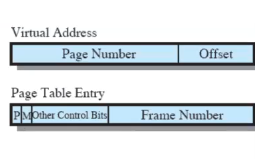
\includegraphics[width=0.65\textwidth]{immagini/pagetableentry}
        \caption{Page Table Entry}
        \label{fig:pagetableentry}
    \end{figure}
    Per quanto riguarda invece l'hardware per la traduzione degli indirizzi, la somma non é una semplice somma: il numero
    di pagina va moltiplicato per il numero di bytes di ogni singola entry della tabella delle pagine, dopo di che si puó
    fare la somma.
    \begin{figure}[H]
        \centering
        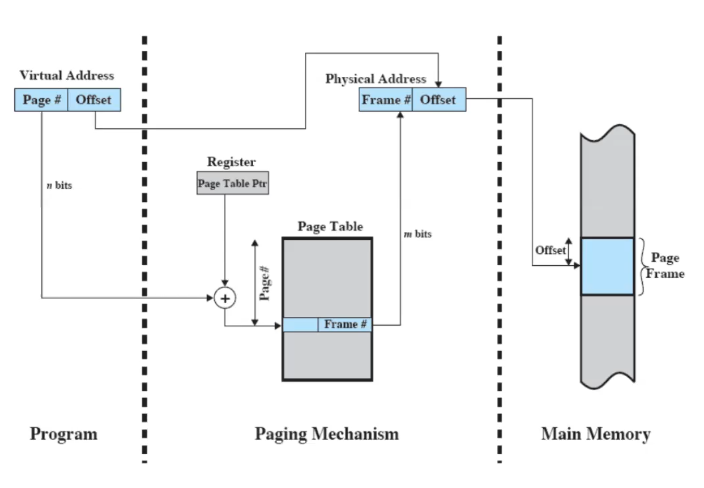
\includegraphics[width=0.65\textwidth]{immagini/HardwarePerPaginazione}
        \caption{Hardware Paginazione}
        \label{fig:hardwarepaginazione}
    \end{figure}
    Il sistema operativo deve :
    \begin{itemize}
        \item caricare a partire da un certo indirizzo / tabella delle pagine del processo
        \item caricare il valore di I in un opportuno registro dipendente dall'hardware
        \item questo va fatto per ogni process switch quindi fa sempre parte del passo 6
    \end{itemize}
    \subsubsection*{Tabelle delle pagine}
    Uno dei problemi é un overhead, perché le tabelle potrebbero contenere molti elmenti, quando un processo é in esecuzione
    , viene assicurato che almeno una parte della sua tabella sia in memoria principale. \\
    
    Esempio:
    \begin{itemize}
        \item Abbiamo 8GB di spazio virtuale, 1KB per pagina, \begin{math}2^23\end{math} entries per ogni tabella delle pagine, ovvero per ogni processo
        \item Con max 4GB di RAM, abbiamo 4 byte
        \item 4 byte per ogni entry 2^2^3=32MB per ogni processo
        \item quindi con 1 RAM di 1GB, bastano 20 processi per occupare piú della metá della memoria con sole strutture di
        overhead
    \end{itemize}
    \subsubsection*{Tabella delle pagine a 2 livelli}
    Per risolvere il problema dell'overhead, si puó usare una tabella delle pagine a 2 livelli, in cui la tabella delle
    pagine é divisa in due parti, la prima parte é una tabella di primo livello, che punta a delle tabelle di secondo livello
    \begin{Figure}
        \centering
        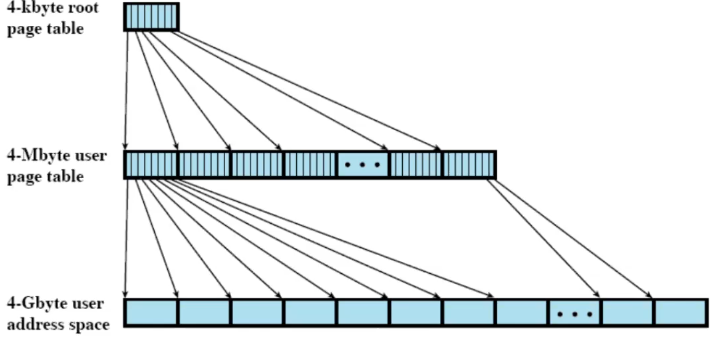
\includegraphics[width=0.65\textwidth]{immagini/TabellaA2Livelli}
        \caption{Tabella delle pagine a 2 livelli}
    \end{Figure}
    In questo caso l'indirizzo virtuale é diviso in 3 parti, la prima parte é usata per indicizzare la tabella di primo livello,
    la seconda parte é usata per indicizzare la tabella di secondo livello, e la terza parte é usata per indicizzare
    la pagina, in questo modo si riduce l'overhead.
    \begin{figure}
        \centering
        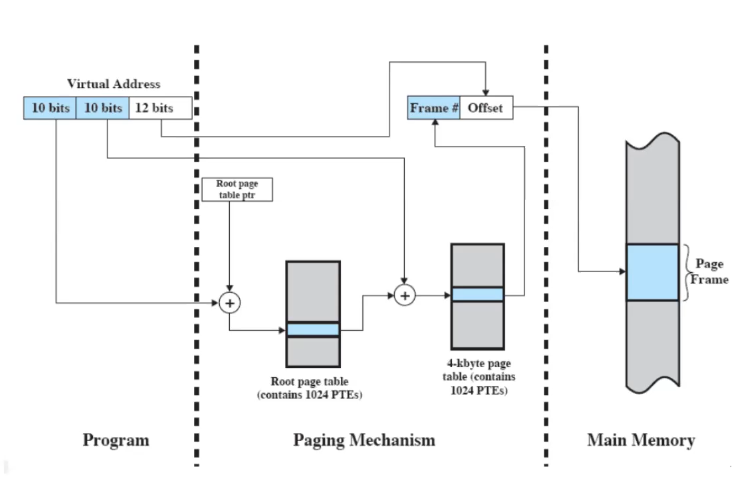
\includegraphics[width=0.65\textwidth]{immagini/HardwareTabella2Livelli}
        \caption{Hardware Tabella delle pagine a 2 livelli}
    \end{figure}
    \subsubsection{Translation Lookaside Buffer}
    IL TLB (memoria temporanea per la traduzione futura), ogni riferimento alla memoria virtuale puó generare
    due accessi alla memoria, si usa un cache veloce per gli elementi delle tabelle delle pagine.
    \subsubsection*{come funziona}
    Dato un indirizzo virtuale, il processore esamina il TLB, se l'indirizzo é presente, il TLB restituisce l'indirizzo
    altrimenti si prende la normale tabella delle pagine del processo,se la pagina risulta in memoria principale, si
    aggiorna il TLB, se la pagina non é in memoria principale, si genera un page fault e si carica in memoria ed infine
    viene aggiornato il TLB usando un algoritmo di sostituzione (LRU tipicamente).
    \begin{figure}[H]
        \centering
        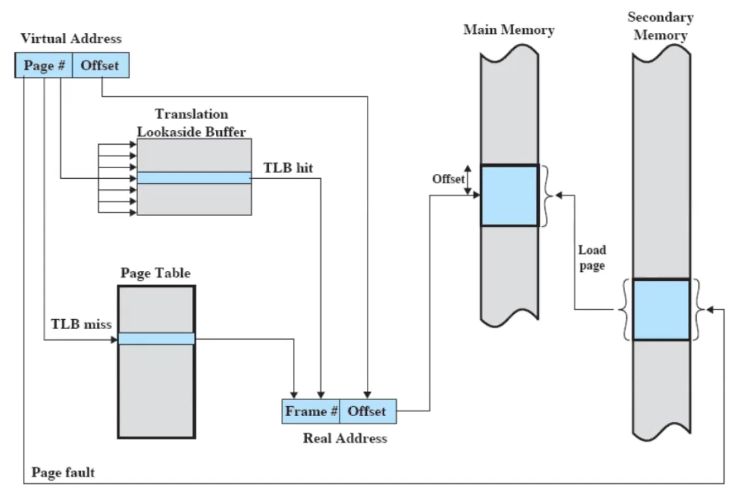
\includegraphics[width=0.65\textwidth]{immagini/HardwareTLB}
        \caption{TLB}
    \end{figure}
    \begin{figure}[H]
        \centering
        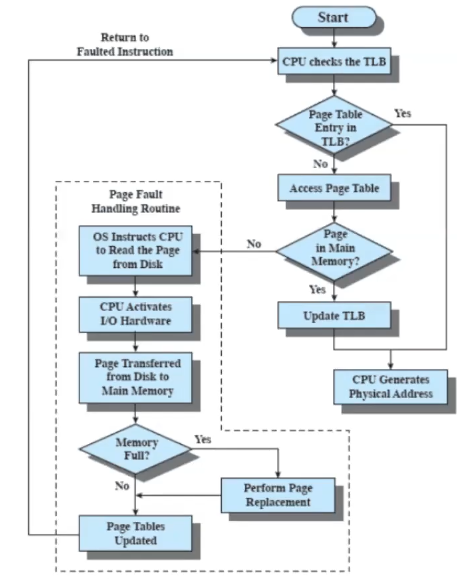
\includegraphics[width=0.65\textwidth]{immagini/FunzionamentoTLB}
        \caption{TLB}
    \end{figure}
    Il sistema operativo deve poter resettare il TLB, perché il TLB contiene informazioni di un processo, e se il processo
    cambia, il TLB deve essere resettato, alcuni processori permettono di avere il PID nel TLB, in modo da invalidare solo alcune
    parti del TLB, é comunque necessario anche senza TLB dire al processore dove é la nuova tabella delle pagine.
    \subsubsection*{Mapping Associativo}
    La tabella delle pagine ha tutte le entry, il TLB contiene solo alcune entry, quindi il numero della pagina non puó essere
    usato direttamente come indice per il TLB (possibile nella tabella delle pagine), Il SO inoltre puó interrogare piú
    elementi del TLB contemporaneamente per capire se c'é o no un hit \textbf{con il supporto hardware}, un altro
    problema é che bisogna fare in modo che il TLB contenga solo pagine in RAM, perché se ci fosse un page fault dopo
    un hit del TLB potremmo non accorgercene, quindi ogni volta che si swappa una pagina bisogna anche resettare o parzilemente il
    TLB.
    \begin{figure}[H]
        \centering
        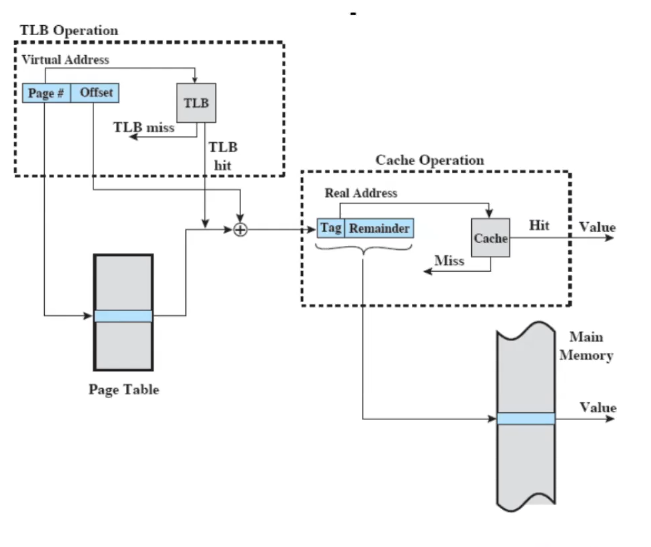
\includegraphics[width=0.65\textwidth]{immagini/TLBeCache}
        \caption{Mapping Associativo}
    \end{figure}
    \subsubsection{Dimensione delle pagine}
    Piú piccola é la pagina, minore é la frammentazione interna, ma maggiore é l'overhead, perché ci sono piú entry,
    la memoria secondaria é ottimizzata per trasferire grossi blocchi di dati, quindi avere le pagine ragionevolmente grandi
    non sarebbe male, quindi piú piccola é una pagina, maggiore il numero di pagine in RAM, E in tutte queste pagine, i riferimenti
    saranno vicini: in accordo con la localitá, i page fault saranno piú rari.
    \subsubsection*{Pagefault vs Dimensione delle pagine}
    \begin{figure}[H]
        \centering
        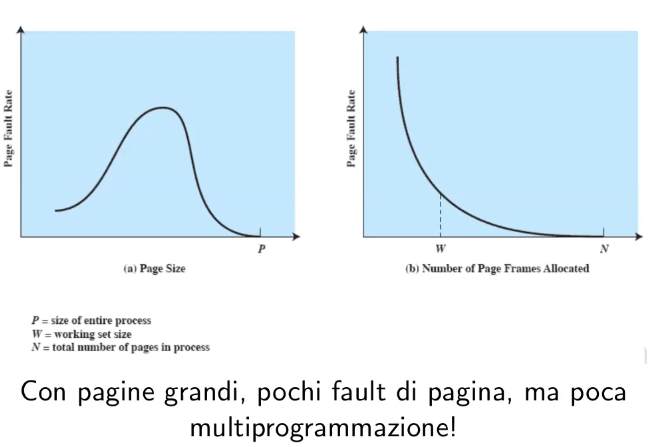
\includegraphics[width=0.65\textwidth]{immagini/Grafico1}
        \caption{Pagefault vs Dimensione delle pagine}
    \end{figure}
    Nelle moderne architetture HW possono supportare pagine anche fino ad 1GB, il sistema operativo
    ne sceglie 1 Es. Linux sugli x86 usa 4KB e le dimensioni piú grandi sono usati in sistemi operativi di grandi architetture
    clustes \ldotsecc ma anche per i sistemi operativi stessi(kernel Mode)












































